\section{Auswertung}
\label{sec:Auswertung}

\subsection{Bestimmung der Heizraten}

Zur Bestimmung der Heizrate $H$ wird der Temperaturgradient zwischen den jeweiligen Messschritten gemittelt:

\begin{equation}
  H = \frac{ \sum_{k=0}^{k_\text{max}} |T(t_{k+1}) - T(t_k)|}{k_\text{max}} \frac{\si{\kelvin}}{\si{\minute}} \; .
\end{equation}

Die Heizraten der beiden Messreihen ergeben sich also zu

\begin{align*}
  H_1 &= \SI{1.60 +- 0.28}{\kelvin\per\minute} \\
  H_2 &= \SI{1.65 +- 0.25}{\kelvin\per\minute} \; .
\end{align*}

\subsection{Bestimmung der Aktivierungsenergie $W$ nach der Approximationsmethode}

Die Messdaten der beiden Messreihen sind in den Tabellen \ref{tab:mess1} und \ref{tab:mess2} aufgeführt.
In den Abbildungen \ref{fig:plot1} und \ref{fig:plot2} wird der Depolarisationsstrom $I$ natürlich logarithmiert und in Abhängigkeit der Temperatur $T$
aufgetragen.

Zur Bestimmung der Aktivierungsenergie $W$ werden die Graphen in den Temperaturintervallen

\begin{align*}
  I_1 &= [\SI{}{\celsius}, \; \SI{}{\celsius}] \\
  I_2 &= [\SI{}{\celsius}, \; \SI{}{\celsius}]
\end{align*}

gemäß der Exponentialfunktion 

\begin{equation}
  f(x) = b \cdot \text{e}^{\sfrac{a}{x}}
\end{equation}

mittels der Funktion \textit{scipy.optimize.curve\_fit} aus der Python-Bibliothek SkiPy genähert.

Die Fitparameter $a$ in den Exponenten ergeben sich also zu

\begin{align*}
  a_1 &= \num{} \\
  a_2 &= \num{}  \; .
\end{align*}

Durch den Vergleich mit Gleichung \eqref{eqn:exp} ergeben sich die Aktivierungsenergien

\begin{align*}
  W_1 &= -a_1 \cdot k_\text{B} = \SI{}{\eV} \\
  W_2 &= -a_2 \cdot k_\text{B} = \SI{}{\eV}  \; .
\end{align*}


\begin{figure}
  \centering
  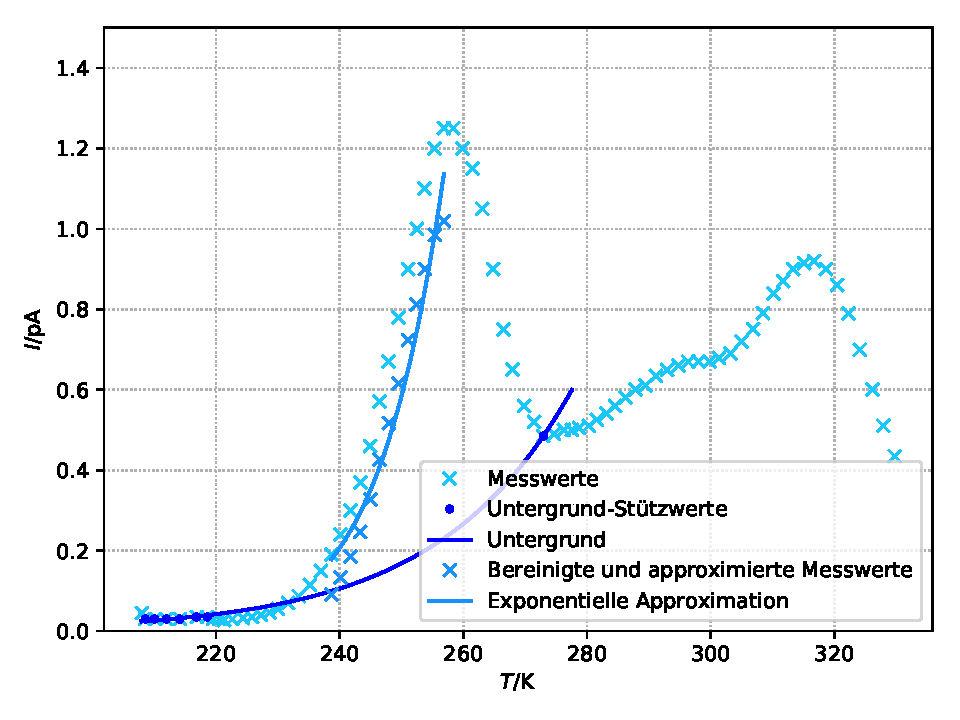
\includegraphics[scale=0.7]{content/plot1.pdf}
  \caption{Exponentiell gefittete $I(T)$-Messwerte mit der Heizrate $H_1 = \SI{1.60 +- 0.28}{\kelvin\per\minute}$}
  \label{fig:plot1}
\end{figure}

\begin{figure}
  \centering
  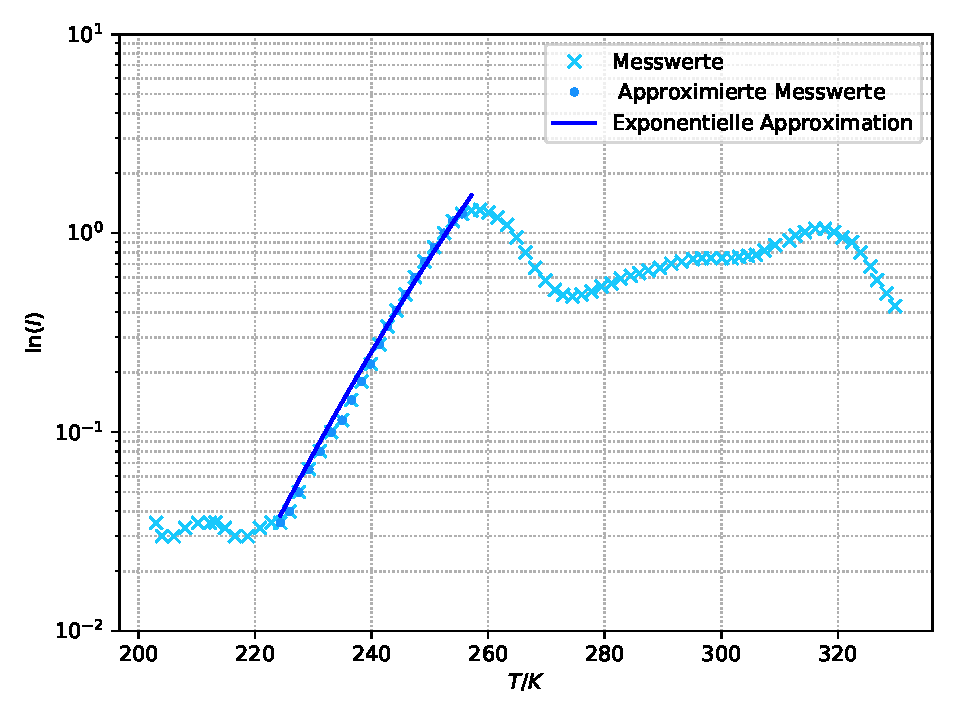
\includegraphics[scale=0.7]{content/plot2.pdf}
  \caption{Exponentiell gefittete $I(T)$-Messwerte mit der Heizrate $H_2 = \SI{1.65 +- 0.25}{\kelvin\per\minute}$}
  \label{fig:plot2}
\end{figure}


\begin{table}
  \centering
  \caption{Messwerte der Temperatur $T$ und des Depolarisationsstromes $I(T)$ in Abhängigkeit von der Zeit $t$ für eine
  Heizrate von $H_1= \SI{999}{\kelvin\per\minute}$}
  \label{tab:mess1}
  \sisetup{table-format=2.1}
  \begin{tabular}{c c c c c c}
  \toprule
  $t \;/\; \si{\minute}$ & $T \;/\; \si{\celsius}$ & $I(T) \;/\; \SI{e-11}{\ampere}$ & 
  $t \;/\; \si{\minute}$ & $T \;/\; \si{\celsius}$ & $I(T) \;/\; \SI{e-11}{\ampere}$ \\
  \midrule
      0 & -65,2 & -0,045 & 39 & -5,2 & -0,650 \\
      1 & -64,6 & -0,030 & 40 & -3,3 & -0,560 \\
      2 & -63,1 & -0,030 & 41 & -1,7 & -0,520 \\
      3 & -61,2 & -0,030 & 42 & -0,2 & -0,485 \\
      4 & -59,0 & -0,030 & 43 &  1,5 & -0,490 \\
      5 & -56,3 & -0,035 & 44 &  3,1 & -0,500 \\
      6 & -54,6 & -0,035 & 45 &  4,4 & -0,500 \\
      7 & -53,6 & -0,030 & 46 &  5,6 & -0,505 \\
      8 & -52,6 & -0,030 & 47 &  7,1 & -0,510 \\
      9 & -51,8 & -0,028 & 48 &  8,4 & -0,525 \\
     10 & -50,5 & -0,030 & 49 & 10,0 & -0,540 \\
     11 & -48,8 & -0,032 & 50 & 11,4 & -0,560 \\
     12 & -47,3 & -0,035 & 51 & 13,1 & -0,580 \\
     13 & -45,9 & -0,040 & 52 & 14,7 & -0,600 \\
     14 & -44,5 & -0,047 & 53 & 16,3 & -0,610 \\
     15 & -43,2 & -0,055 & 54 & 18,0 & -0,635 \\
     16 & -41,5 & -0,070 & 55 & 19,8 & -0,650 \\
     17 & -39,8 & -0,087 & 56 & 21,6 & -0,660 \\
     18 & -38,0 & -0,115 & 57 & 23,2 & -0,670 \\
     19 & -36,2 & -0,150 & 58 & 24,9 & -0,670 \\
     20 & -34,5 & -0,190 & 59 & 26,7 & -0,670 \\
     21 & -33,0 & -0,240 & 60 & 28,2 & -0,680 \\
     22 & -31,4 & -0,300 & 61 & 30,1 & -0,690 \\
     23 & -29,8 & -0,370 & 62 & 31,8 & -0,720 \\
     24 & -28,2 & -0,460 & 63 & 33,7 & -0,750 \\
     25 & -26,7 & -0,570 & 64 & 35,3 & -0,790 \\
     26 & -25,2 & -0,670 & 65 & 37,0 & -0,840 \\
     27 & -23,6 & -0,780 & 66 & 38,6 & -0,870 \\
     28 & -22,1 & -0,900 & 67 & 40,2 & -0,900 \\
     29 & -20,7 & -1,000 & 68 & 42,0 & -0,915 \\
     30 & -19,4 & -1,100 & 69 & 43,6 & -0,920 \\
     31 & -17,8 & -1,200 & 70 & 45,5 & -0,900 \\
     32 & -16,3 & -1,250 & 71 & 47,3 & -0,860 \\
     33 & -14,8 & -1,250 & 72 & 49,1 & -0,790 \\
     34 & -13,3 & -1,200 & 73 & 51,0 & -0,700 \\
     35 & -11,7 & -1,150 & 74 & 53,0 & -0,600 \\
     36 & -10,1 & -1,050 & 75 & 54,8 & -0,510 \\
     37 &  -8,3 & -0,900 & 76 & 56,6 & -0,435 \\
     38 &  -6,7 & -0,750 &    &      &        \\ 
  \bottomrule
  \end{tabular}
  \end{table}

  \begin{table}
    \centering
    \caption{Messwerte der Temperatur $T$ und des Depolarisationsstromes $I(T)$ in Abhängigkeit von der Zeit $t$ für eine
    Heizrate von $H_2= \SI{999}{\kelvin\per\minute}$}
    \label{tab:mess2}
    \sisetup{table-format=2.1}
    \begin{tabular}{c c c c c c}
    \toprule
    $t \;/\; \si{\minute}$ & $T \;/\; \si{\celsius}$ & $I(T) \;/\; \SI{e-11}{\ampere}$ & 
    $t \;/\; \si{\minute}$ & $T \;/\; \si{\celsius}$ & $I(T) \;/\; \SI{e-11}{\ampere}$ \\
    \midrule
        0 & -70,1 & -0,035 & 39 & -5,1 & -0,670 \\
        1 & -69,1 & -0,030 & 40 & -3,3 & -0,580 \\
        2 & -67,1 & -0,030 & 41 & -1,7 & -0,520 \\
        3 & -65,1 & -0,033 & 42 & -0,3 & -0,490 \\
        4 & -62,9 & -0,035 & 43 &  1,3 & -0,480 \\
        5 & -60,9 & -0,035 & 44 &  2,9 & -0,490 \\
        6 & -59,9 & -0,035 & 45 &  4,6 & -0,510 \\
        7 & -58,3 & -0,033 & 46 &  6,3 & -0,540 \\
        8 & -56,6 & -0,030 & 47 &  8,0 & -0,560 \\
        9 & -54,4 & -0,030 & 48 &  9,6 & -0,590 \\
       10 & -52,3 & -0,033 & 49 & 11,3 & -0,610 \\
       11 & -50,3 & -0,035 & 50 & 12,8 & -0,630 \\
       12 & -48,8 & -0,035 & 51 & 14,3 & -0,650 \\
       13 & -47,2 & -0,040 & 52 & 16,3 & -0,670 \\
       14 & -45,6 & -0,050 & 53 & 18,3 & -0,700 \\
       15 & -43,9 & -0,065 & 54 & 20,1 & -0,720 \\
       16 & -42,0 & -0,080 & 55 & 22,0 & -0,740 \\
       17 & -40,1 & -0,100 & 56 & 23,6 & -0,750 \\
       18 & -38,2 & -0,115 & 57 & 25,1 & -0,750 \\
       19 & -36,6 & -0,145 & 58 & 27,0 & -0,750 \\
       20 & -34,9 & -0,180 & 59 & 28,6 & -0,750 \\
       21 & -33,3 & -0,220 & 60 & 29,9 & -0,760 \\
       22 & -31,8 & -0,275 & 61 & 31,4 & -0,770 \\
       23 & -30,4 & -0,340 & 62 & 32,8 & -0,780 \\
       24 & -28,9 & -0,410 & 63 & 34,3 & -0,820 \\
       25 & -27,3 & -0,490 & 64 & 36,1 & -0,870 \\
       26 & -25,7 & -0,600 & 65 & 38,6 & -0,920 \\
       27 & -24,0 & -0,720 & 66 & 39,6 & -0,970 \\
       28 & -22,4 & -0,850 & 67 & 41,2 & -1,010 \\
       29 & -20,7 & -1,000 & 68 & 43,0 & -1,050 \\
       30 & -19,2 & -1,150 & 69 & 44,6 & -1,050 \\
       31 & -17,6 & -1,250 & 70 & 46,2 & -1,010 \\
       32 & -16,0 & -1,300 & 71 & 47,7 & -0,950 \\
       33 & -14,5 & -1,310 & 72 & 49,3 & -0,900 \\
       34 & -13,1 & -1,270 & 73 & 50,8 & -0,800 \\
       35 & -11,5 & -1,200 & 74 & 52,4 & -0,680 \\
       36 &  -9,9 & -1,100 & 75 & 53,6 & -0,580 \\
       37 &  -8,3 & -0,950 & 76 & 55,2 & -0,500 \\
       38 &  -6,7 & -0,800 &    & 56,7 & -0,430 \\ 
    \bottomrule
    \end{tabular}
    \end{table}
